\section{Evaluation and Results}
\label{sec:results}

Table~\ref{tab:results} reports validation performance; all \NRunTotal{} runs
completed successfully and none read the test block.

% GENERATED by scripts/build_latex_assets.py -- do not edit by hand.
% Source: experiments/models/*/*/metrics.json (validation split only).
\begin{table}[t]
\centering
\caption{Validation performance for each model family under the shared protocol (variant P2, standardised inputs, seed 42). Skill is measured against naive persistence on identical forecast dates. Absolute errors are in quote currency and are \emph{not} comparable between AAPL and BTC; only the unitless skill column is. The test block was not used.}
\label{tab:results}
\small
\setlength{\tabcolsep}{4pt}
\begin{tabular}{@{}l r r r r r r@{}}
\toprule
 & \multicolumn{3}{c}{AAPL} & \multicolumn{3}{c}{BTC} \\
\cmidrule(lr){2-4}\cmidrule(l){5-7}
Model & MAE & RMSE & Skill & MAE & RMSE & Skill \\
\midrule
Linear baseline & 2.92 & 4.37 & \textbf{-0.50} & 1603.59 & 2211.24 & +0.05 \\
Ridge & 2.90 & 4.36 & +0.29 & 1602.39 & 2205.96 & +0.12 \\
SVR (RBF) & 2.89 & 4.36 & +0.52 & 1603.13 & 2203.85 & +0.08 \\
Random forest & 2.93 & 4.37 & \textbf{-0.78} & 1603.37 & 2208.04 & +0.06 \\
Hist.\ gradient boosting & 2.90 & 4.36 & +0.25 & 1605.02 & 2204.91 & \textbf{-0.04} \\
\midrule
Naive persistence & 2.91 & 4.36 & 0.00 & 1604.35 & 2205.67 & 0.00 \\
\bottomrule
\end{tabular}
\par\smallskip\footnotesize
Skill is $1 - \mathrm{MAE}_{\mathrm{model}}/\mathrm{MAE}_{\mathrm{naive}}$ in percent; negative values (bold) are worse than the baseline. $n=244$ (AAPL) and $358$ (BTC) validation sessions.
\end{table}


\paragraph{RQ1: nothing meaningfully beats persistence.}
The best result is \BestAAPLModel{} on AAPL at \BestAAPLSkill\% skill and
\BestBTCModel{} on BTC at \BestBTCSkill\% --- a fraction of a percentage point
above doing nothing. Two models are worse: the random forest on AAPL
(\SkillAAPLRandomForest\%) and the boosted ensemble on BTC
(\SkillBTCHistGradientBoosting\%).
\begin{figure}[t]
  \centering
  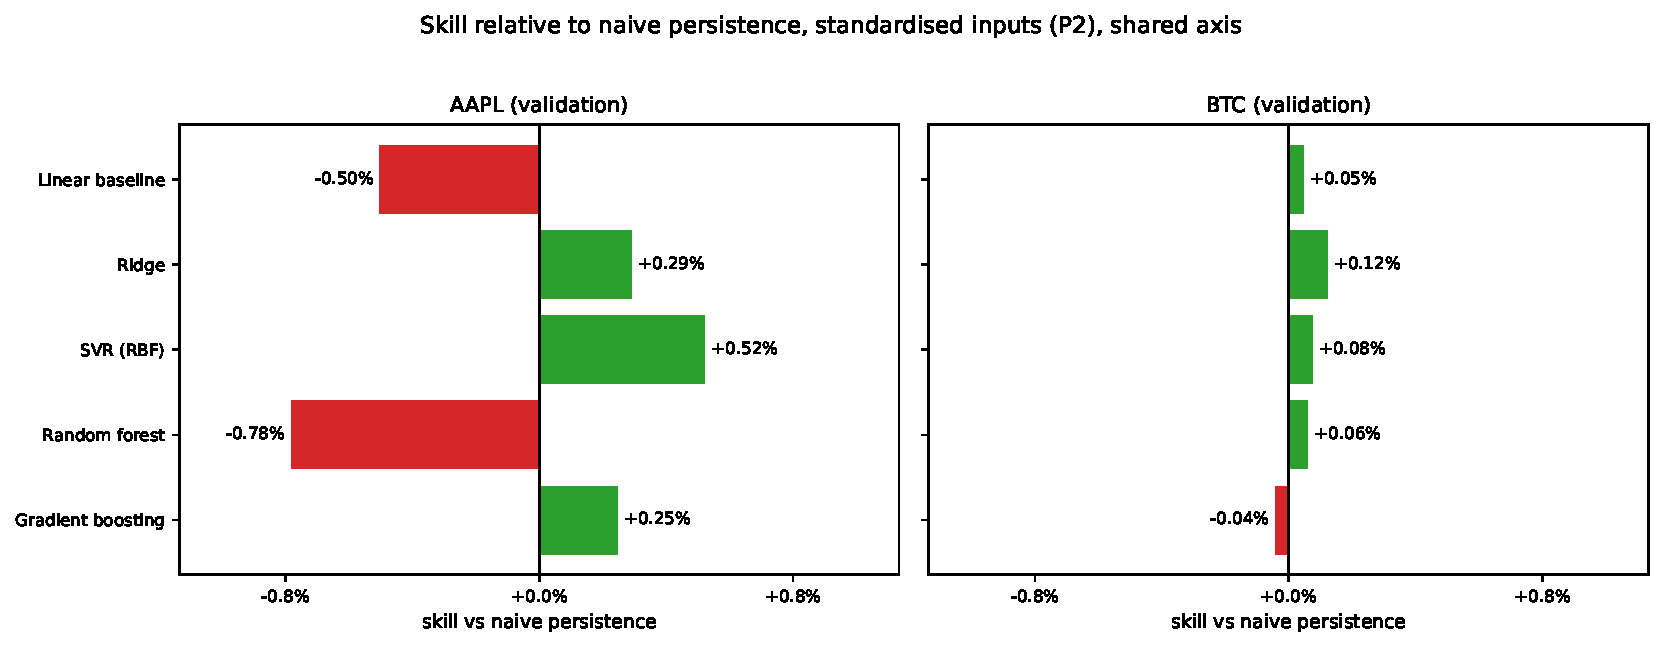
\includegraphics[width=\linewidth]{figures/fig04_model_vs_naive.pdf}
  \caption{Skill relative to naive persistence, per asset, on a \emph{shared}
  horizontal axis. Sharing matters: per-panel autoscaling would make BTC's
  fraction of a percent look as large as AAPL's. Bars left of zero are worse than
  repeating the current price.}
  \label{fig:skill}
\end{figure}

\paragraph{RQ2: capacity and regimes.}
Figure~\ref{fig:assets} gives the mechanical explanation: BTC's volatility is
higher and more variable, so a model with capacity fixed by an identical budget
faces a harder target, and every BTC skill value is closer to zero. On AAPL, where
capacity has more room to matter, the most flexible ensemble does worst --- the
signature of fitting noise.

\begin{figure}[t]
  \centering
  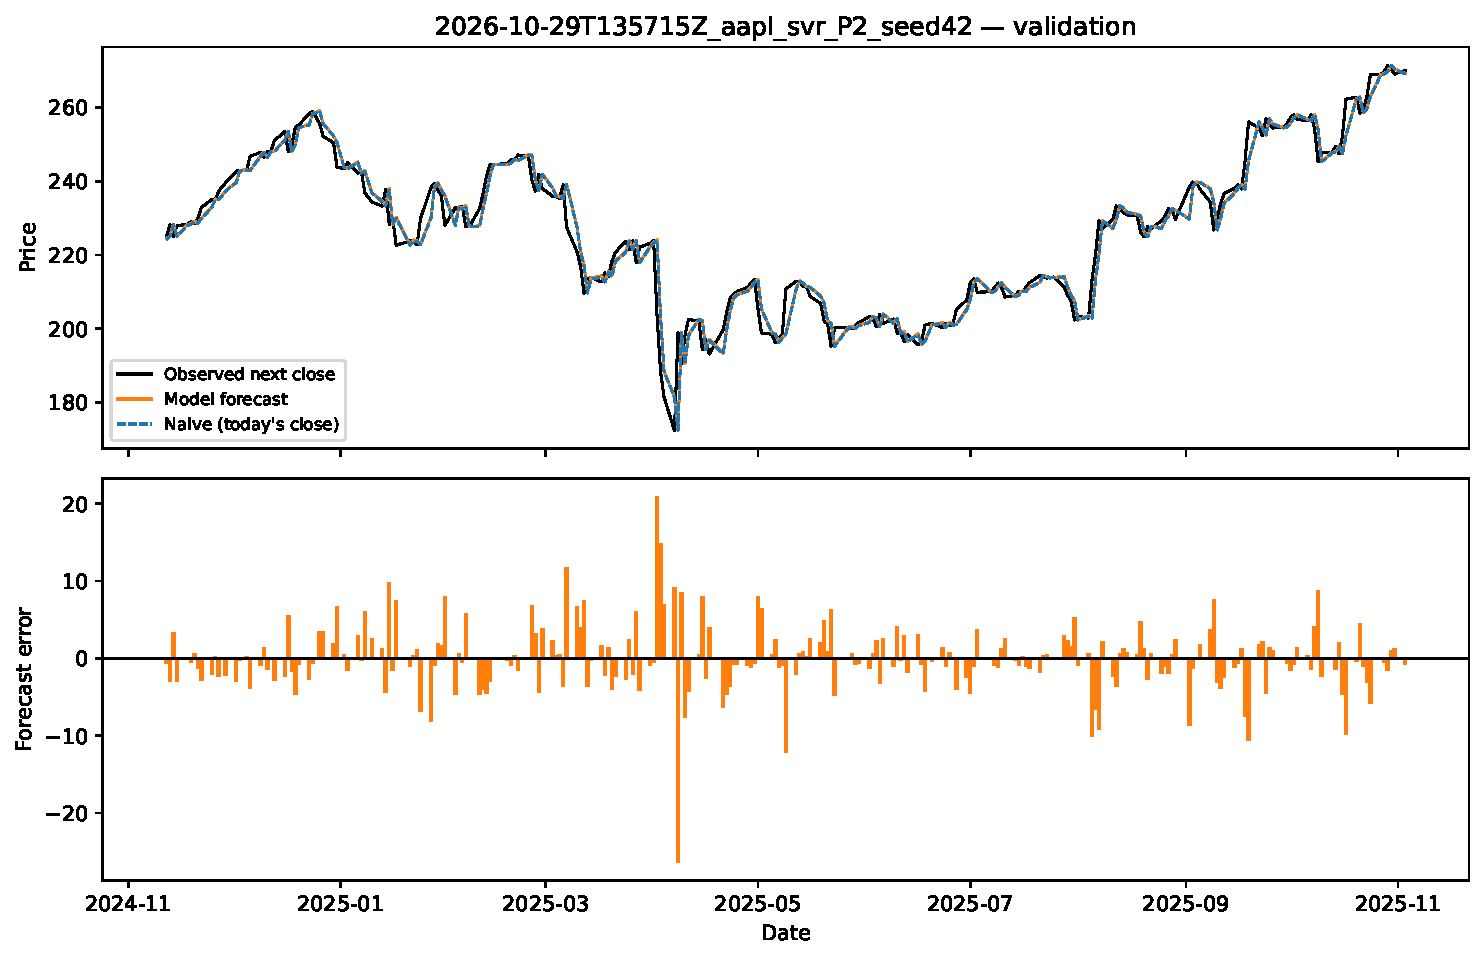
\includegraphics[width=0.78\linewidth]{figures/fig03_observed_vs_predicted_2026-10-29T135715Z_aapl_svr_P2_seed42_validation.pdf}
  \caption{Observed next close against the fitted SVR and naive forecasts on the
  AAPL validation block, with signed error below. The naive line tracks the
  observed series closely, which is why absolute error is a poor way to judge a
  model and skill is used instead.}
  \label{fig:forecast}
\end{figure}

\paragraph{Why they fail.}
The explanation is statistical, not architectural: daily return autocorrelation is
close to zero, so the features carry little information about the next session's
direction and extra parameters fit noise. The forest adds a structural limit ---
its predictions average leaf values, so it cannot extrapolate. Since all skill values lie within about one percentage point and the middle
ranking changes between assets, we claim no family is superior: the conclusion is
a tie against the baseline.

\begin{figure}[t]
  \centering
  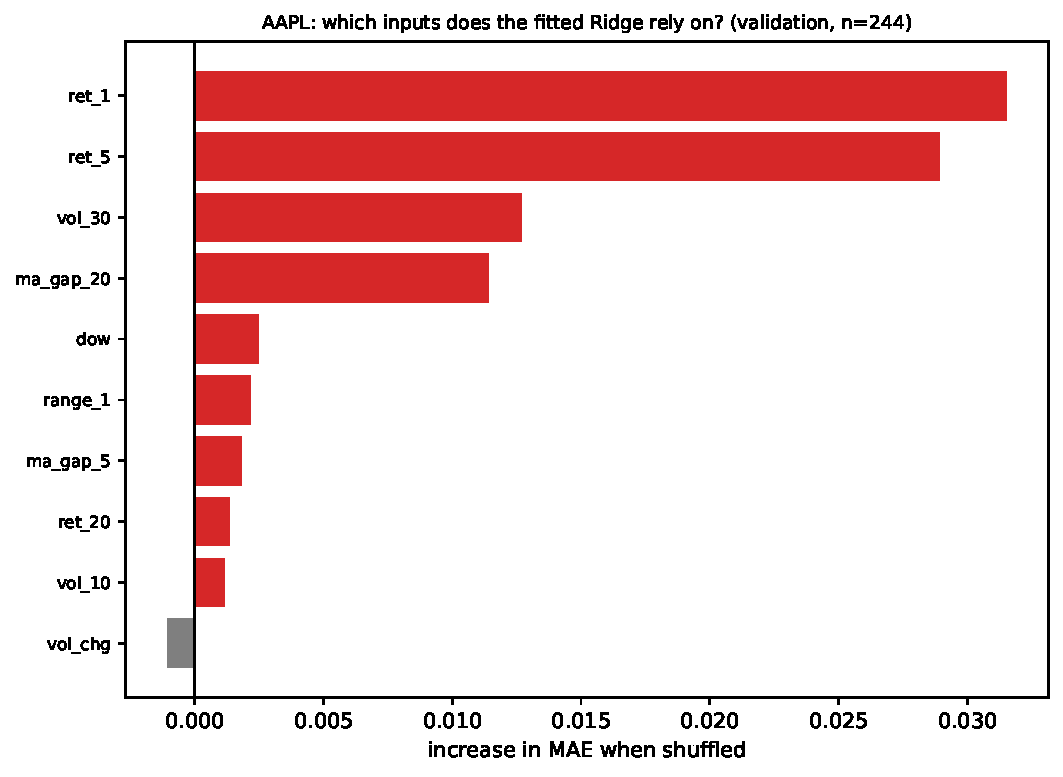
\includegraphics[width=0.76\linewidth]{figures/fig07_feature_importance_aapl.pdf}
  \caption{Learner-facing interpretability: permutation importance for the fitted
  Ridge model on the AAPL validation block, measured as the increase in MAE when
  one feature is shuffled \citep{fisher2019allmodels}. The model relies most on short-horizon returns and
  trailing volatility, and the magnitudes are tiny --- consistent with the skill
  table. This describes the fitted model, not a causal claim about markets.}
  \label{fig:importance}
\end{figure}
